\chapter{Módulo de controle de infusão de insulina}
\label{cap:oraganizacao_software}
Módulo desenvolvido é responsável por controlar o funcionamento da bomba em função dos parâmetros recebidos e pré estabelecidos. É possível configurar a quantidade a ser infundido no período de 24 horas, infusão basal, e, além disso e mais importante, o desenvolvimento foi feito em cima do simulador proteus e devido a possibilidade de mudanças possíveis o sistema foi montado de forma que deixa os módulos desacoplados. Para isso foi utilizado o conceito OOC, \emph{Object Orientated Programming in ANSI-C}, o que possibilitou o uso de \emph{Design Patterns}.

\section{Proteus}

No desenvolvimento deste TCC o simulador Proteus foi usado para montar o ambiente de tesste. Para testes, o circuito teve seu desenvolvimento em função dos seguintes componentes: microcontrolador da família PIC, PIC18F452, motor de passo, \emph{display} de LCD 2x16, botões e driver para o motor de passo. A Figura \ref{fig:proteus} representa a imagem do \emph{Software}.

\begin{figure}[htp]
	\centering
	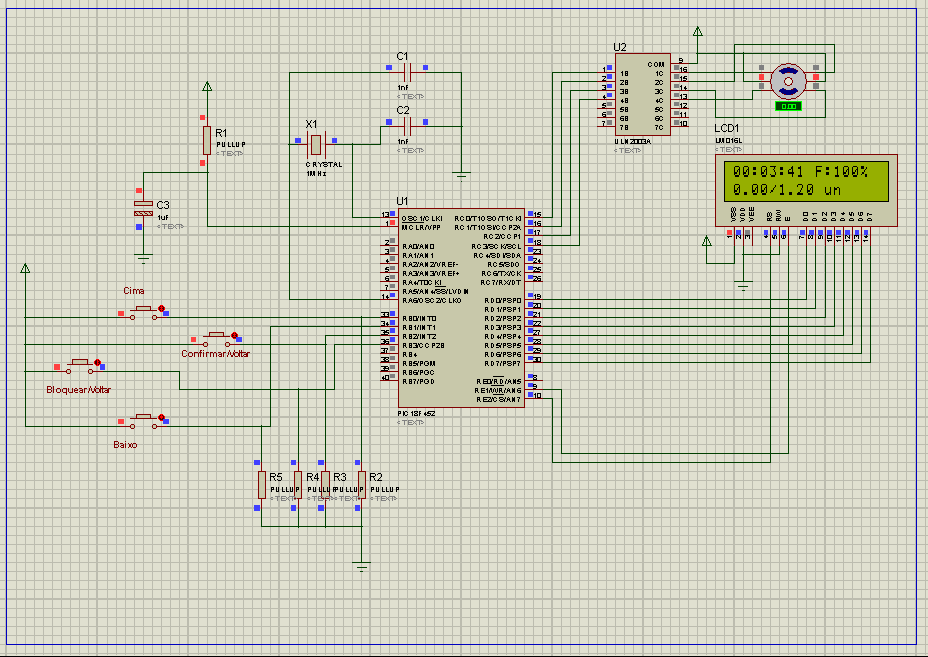
\includegraphics[scale=0.5]{images/proteus.png}
	\caption{\emph{Software} Proteus}	
	\label{fig:proteus}
\end{figure}

\section{Arquitetura do Software}

O \emph{Software} foi desenvolvido de forma modular para que as funções fossem facilmente testadas, modificadas e evoluídas, a Figura \ref{fig:arquiteturageral} representa a estrutura citada. A divisão do \emph{Software} foi feita da seguinte forma: config, insulimpump, lcd, menu, motor, timerMotor e principal. 

\begin{figure}[htp]
	\centering
	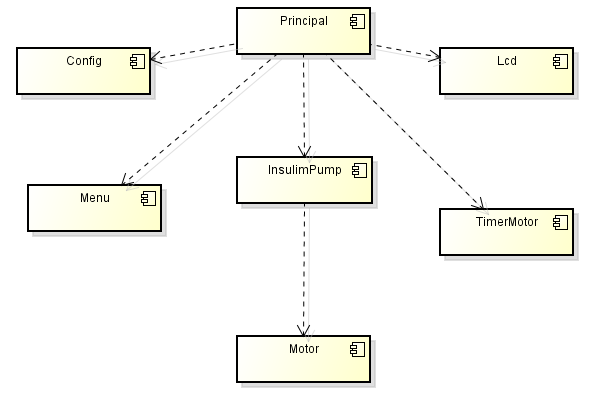
\includegraphics[scale=0.7]{images/arquitetura.png}
	\caption{Estrutura do \emph{Software}}	
	\label{fig:arquiteturageral}
\end{figure}

\subsection{Módulo Config}

Módulo feito para centralizar todas as configurações do sistema, utilizado, basicamente, por quase todos os demais módulos. Seguindo parte do conceito de OOC, pois foi possível utilizar a ideia de \emph{private} e \emph{public} para as variáveis. Entretanto não foi criada nenhuma \emph{struct} de forma que representasse uma classe. A Figura \ref{fig:driagramaclasseconfig} representa o diagrama de classe desse módulo. \newpage


\begin{figure}[htp]
	\centering
	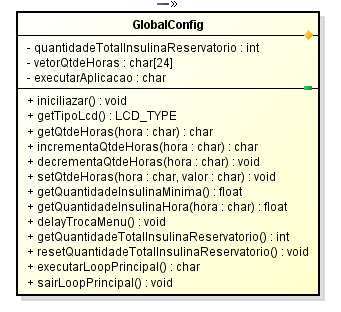
\includegraphics[scale=1]{images/classe_GlobalConfig.png}
	\caption{Diagrama de classe GlobalConfig}	
	\label{fig:driagramaclasseconfig}
\end{figure}

Quando se diz \emph{private} e \emph{public} é o fato de adicionar as variáveis no arquivo GlobalConfig.h, \emph{private}, ou GlobalConfig.c, \emph{public}. A principal parametrização desse módulo é a quantidade que o repositório de insulina suporta. Para modificar seu valor basta alterar o \emph{define} QUANTIDADE\_TOTAL\_RESERVATORIO\_INSULINA. Esse valor representa a quantidade de insulina existente no reservatório na escala da infusão mínima da bomba.

\subsection{Módulo InsulinPump}

O módulo InsulinPump é responsável pela abstração das funções da bomba para o resto do sistema. Funções simples para o resto do sistema como: inicializar variáveis de controle, iniciar operação, parar operação - principalmente para configurações da bomba -, injetar e retornar a quantidade inserida naquela hora. Seguindo o conceito OOC foi criada uma "interface", IInsulinPump, e a "classe" concreta InsulinPump. A Figura \ref{fig:diagramainsulinpump} representa a relação e diagrama de classe dos elementos citados anteriormente.

\begin{figure}[htp]
	\centering
	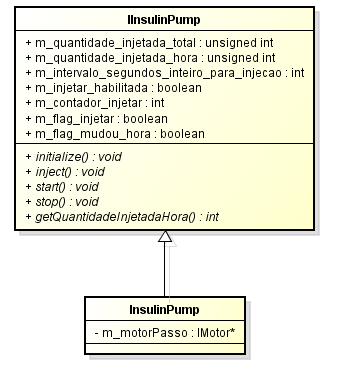
\includegraphics[scale=1]{images/classe_insulinpump.png}
	\caption{Diagrama de classe InsulinPump}	
	\label{fig:diagramainsulinpump}
\end{figure}

\subsection{Módulo Lcd}

Esse módulo é responsável pelo isolamento do \emph{display} de LCD do resto do sistema. Composto por um \emph{factory}, que retorna um obeto de controle de acordo com o parâmetro passado, uma "interface" para possibilitar essa abstração e as classes concretas, no caso existe apenas a classe concreta para \emph{display} 2x16(2 linhas por 16 colunas). A Figura \ref{fig:diagramalcd} representa a relação e diagrama de classe dos elementos citados anteriormente.

\begin{figure}[htp]
	\centering
	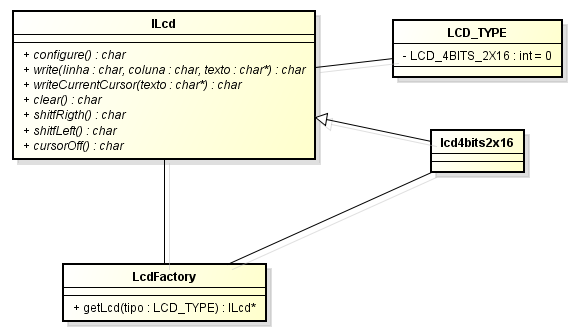
\includegraphics[scale=0.8]{images/classe_lcd.png}
	\caption{Diagrama de classe Lcd}	
	\label{fig:diagramalcd}
\end{figure}

\subsection{Módulo Menu}

O módulo de menu foi criado para abstrair todos as possíveis situações e estados da bomba. Foi criado de uma forma muito simples e é equivalente a uma máquina de estado. Utiliza uma "inteface" que é implementado por todos os tipos de menu existentes como: menu de confuguração da bomba, menu da bomba em execução, menu de confirmação do estado do reservatório e outros. A Figura \ref{fig:classemenu} representa as relações entre os componentes, ou "classes", do módulo e demonstra como é simples a criação de novos menus.

\begin{figure}[htp]
	\centering
	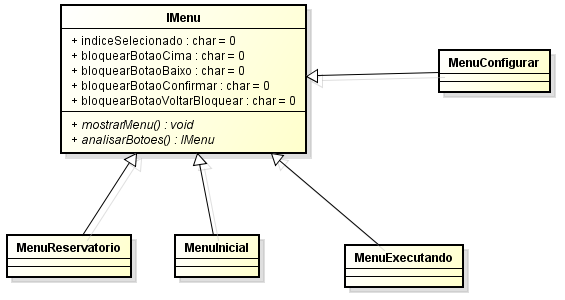
\includegraphics[scale=1]{images/classe_menu.png}
	\caption{Diagrama de classe Menu}	
	\label{fig:classemenu}
\end{figure}

\subsection{Módulo Motor}

O módulo motor, tem como resposabilidade abstrair todas as operações necessárias para o controle do motor de forma que o resto do sistema não saiba qual motor está utilizando. Isso é possível devido a "interface" criada para abstração e o uso de um \emph{Factory} que retorna o motor que deve ser utilizado de acordo com um parâmetro global, localizado no módulo config. A figura \ref{fig:classemotor} representa as relações existentes nesse módulo. \newpage


\begin{figure}[htp]
	\centering
	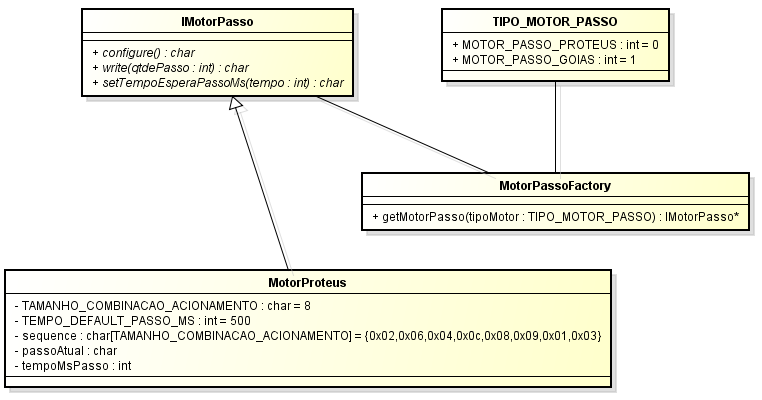
\includegraphics[scale=0.8]{images/classe_motor.png}
	\caption{Diagrama de classe Motor}	
	\label{fig:classemotor}
\end{figure}

\subsection{Módulo TimerMotor}

O módulo TimerMotor armazena todos os dados do contador para o uso dos motores. Abstrai a configuração do timer em função do \emph{hardware} para o resto do sistema. Dessa forma o sistema só precisa se preocupar em: fazer configuração inicial(inicializar variáveis), iniciar timer, parar timer. A Figura \ref{fig:classe_timer_motor} representa a relação citada acima.

\begin{figure}[htp]
	\centering
	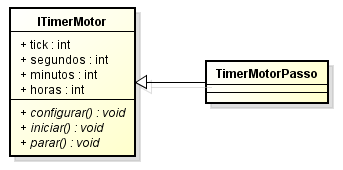
\includegraphics[scale=1]{images/classe_timer_motor.png}
	\caption{Diagrama de classe TimerMotoror}	
	\label{fig:classe_timer_motor}
\end{figure}


\subsection{Módulo Principal}

Devido a forma modular com  que foi implementado o sistema esse tornou-se o módulo mais simples. Ficou responsável apenas pela interrupção, específico do hardware, chamar os métodos de incialização dos módulos do lcd, TimerMotor e InsulinPump, e um loop principal, extremamente simples, que exibe o Menu, correspondente ao estado atual, e recebe o retorno do próprio menu em questão para navegar entre os menus existente.